\section{Data Set Description}
\label{sec:datasetdescription}
This paper will use data from the SAW, which allows us to analyze data from  in total 1695 different systems and more than 50000 snapshots. The data set contains production systems across various industries. Figure \ref{fig:industries} gives an overview about the distribution of systems across industry sectors. Government systems form a very dominant group, which should be taken into account before generalizing the results.

\begin{figure}
\centering
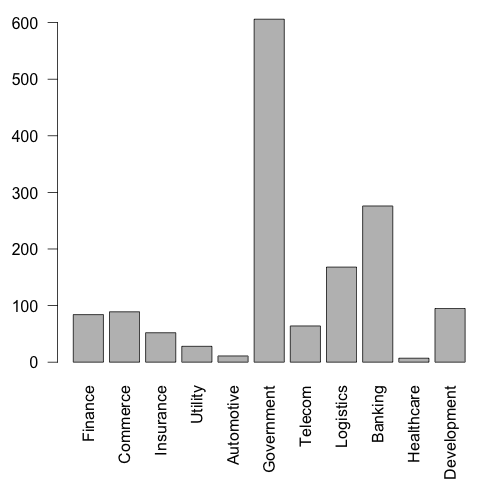
\includegraphics[width=\linewidth]{figs/ind_occ.png}
\caption{Occurrance of industries}
\label{fig:industries}
\end{figure}

Each snapshot contains a set of metrics of a system at a certain point in time as well as some meta-data about the system. The set of metrics contains different types of metrics. For system metrics, three types of code are distinguished, namely production code, generated code and test code. Metrics for these three types of code are available separately. We decided to focus exclusively on metrics that measure production code as this is the code that best represents the systems we want to examine.

Metrics are not only separately available for types of code but also for each involved programming language. These metric sets can contain language-specific metrics. In addition, a set of metrics aggregated across all languages is available. Because our goal targets systems in general, regardless of language, we focused on this set of across-language metrics.

Each system is further subdivided into components and each component into files and if appropriate further down into units (e.g. methods). Because of a limited set of available metrics on file and unit level we disregarded these and component information was only used to a limited extent. We decided so because we observed that component counts can dramatically change during a project, which might be due to refactoring or simply redefining of component structures. These changes make it hard to generally track development of components over time. Also the way components are defined is dependent on the specific system and is not following a concrete schema. That makes it hard to compare components among systems. Because our goal was to generally compare systems, the component structure is interesting though. Some information about structure are also already available as system-level metrics, like e.g. component (volume) balance, component count and language count. The only thing which we derived directly from the components was the set of used programming languages. 

When looking only a system-level metrics, our data-set contains still a large number of different metrics, in total over 1200 different metrics are represented. Figure \ref{fig:metric_occurance} shows the occurrences of metrics in the data-set. Most of the metrics are not usable for our purposes since they only occur a few times. To be able to get data with an acceptable amount of missing values to use with machine learning methods, we focused on extracting the 150 most commonly occurring metrics in the data-set.


\begin{figure}[!htbp]
\begin{minipage}{.45\linewidth}
\centering
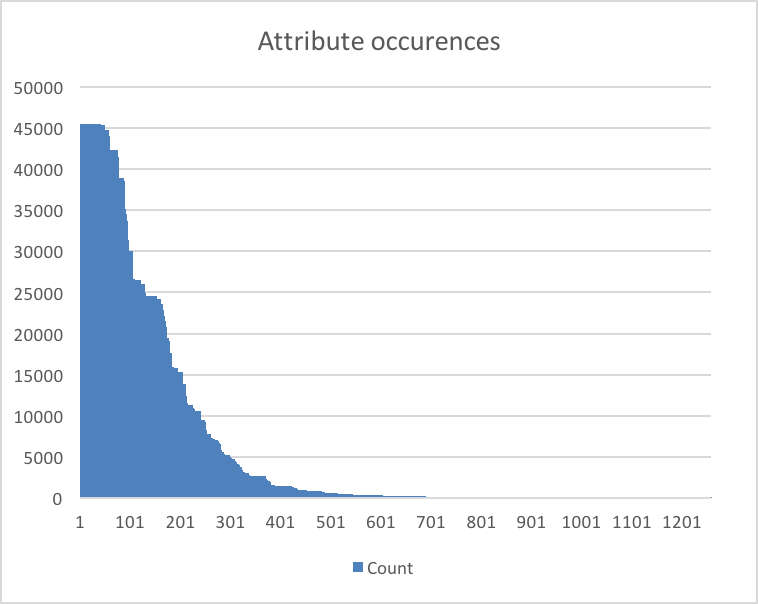
\includegraphics[width=0.9\linewidth, height=0.75\linewidth]{figs/metric_occ.png}
\caption{Number of occurrences of metrics in the data-set}
\label{fig:metric_occurance}
\end{minipage}
\begin{minipage}{.5\linewidth}
\centering
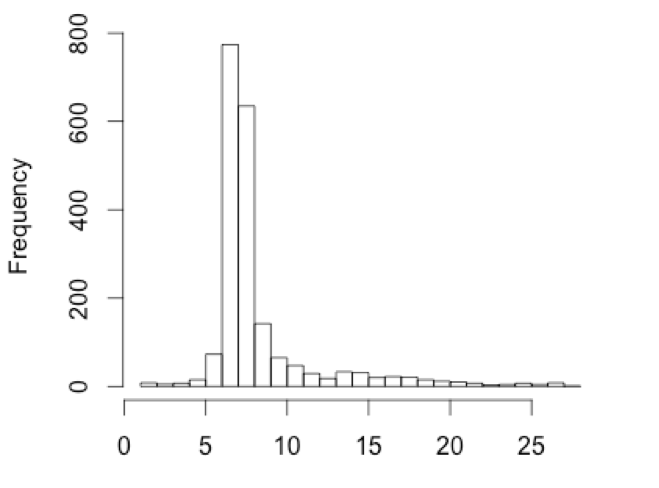
\includegraphics[width=0.9\linewidth, height=0.75\linewidth]{figs/time_snaps.png}
\caption{Temporal distance between snapshots in days}
\label{fig:time_snapshots}
\end{minipage}
\end{figure}

For some systems our data-set only contains one or two snapshots while for others it contains a substantial amount more. These snapshot are not always evenly spaced, some are taken a week apart, some months. When we examined the distribution of the time between snapshots (figure \ref{fig:time_snapshots}) we found that most are taken about a week after the previous snapshots but some are taken many months after the previous snapshot.

\subsection{Snapshots Series}
Systems assessed by SIG are either assessed once or inspected over a certain amount of time, which depends on customer requirements. During the inspection period multiple snapshots of the systems are taken which will be called snapshot series in the following paragraphs.

Snapshots series are not always evenly temporal spaced, most have been taken weekly but some also 2-weekly or with irregular distances. This and other aspects of snapshot series are of interest for later creation of the model. 
Therefore an analysis of the exact structure of the available snapshot series is important and will be outlined in the following. Hereby the arrows in Figure \ref{fig:schema} illustrates which characteristics have been analyzed.

\begin{figure}[!htb]
  \centering
  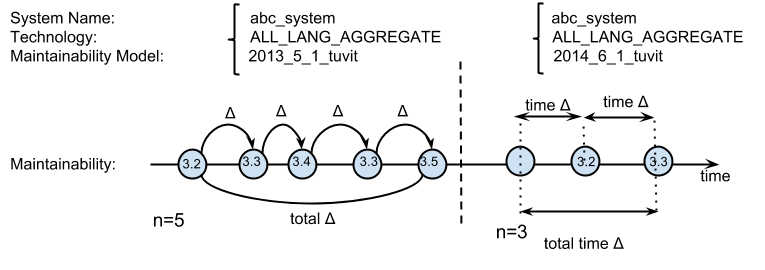
\includegraphics[width=0.8\linewidth]{figs/analysis_schema.png}
  \caption{Snapshot series analysis}
  \label{fig:schema}
\end{figure}

The analysis was done based on measurements from 1687 different software systems. In total, the data set consists of $\sim$50000 snapshots. Figure \ref{fig:series_1} shows the number of snapshots per series (mean=13.96, median=5) and the time distance between single snapshots in a series (mean=8.44). The histograms show that a high number of systems were only measured a few times (1 time: 566, 2 times: 272, 3 times: 196) and that the majority of systems were measured with a temporal distance between 6 and 8 days (6 days: 35, 7 days: 554, 8 days: 21). The right histogram shows that even over the whole period of measurements the vast majority of systems improve/deteriorate by less than 0.5 stars, measurements show that 95\% of the systems change between -0.33 and +0.34 over a period of average 168 days.

\begin{figure}[htb]
\centering
\begin{minipage}{.45\linewidth}
\centering
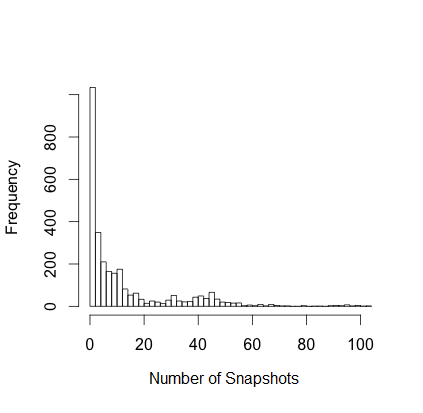
\includegraphics[width=\linewidth]{figs/Rplot__cval.png}
\end{minipage}
\begin{minipage}{.45\linewidth}
\centering
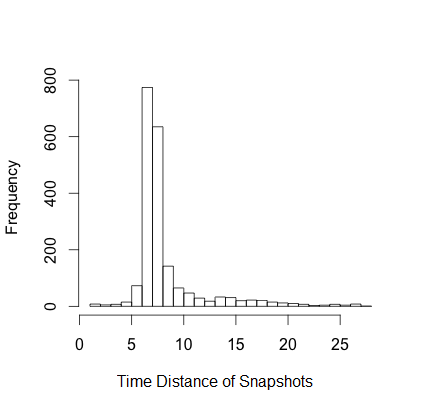
\includegraphics[width=\linewidth]{figs/Rplot__zval.png}
\end{minipage}
\begin{minipage}{.45\linewidth}
\centering
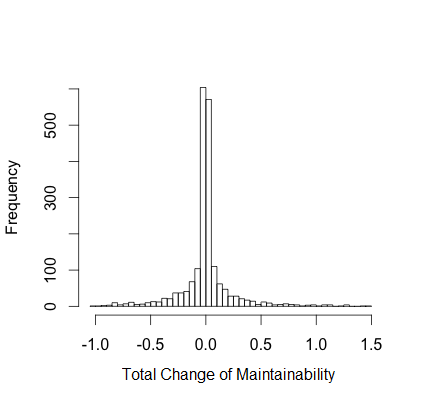
\includegraphics[width=\linewidth]{figs/Rplot__tval.png}
\end{minipage}
\caption{Histograms of: Number of snapshots per series (left, \textless99\% percentile), distance between snapshots in days (middle, \textless85\% percentile) and change of maintainability between start and end of series (right, \textgreater0.5\% percentile \& \textless99.5\% percentile). For a better visualization the plots were cleaned from extreme outlier values.}
\label{fig:series_1}
\end{figure}
 
Also the circumstance of maintainability model changes has to be highlighted. SIG's maintainability model gets periodically (usually yearly) updated and re-calibrated to maintain and improve the accuracy of the model. This is expected to have an impact on the maintainability value and has to be taken into account in further steps. To show the impact of model changes, three long-term monitored systems were selected and the maintainability metric of these systems was plotted over time (see Figure \ref{fig:model_inf}). Hereby the color represents the current model version and the horizontal lines mark model changes. It is clear to see that some model changes seem to cause sudden drops of the maintainability value (e.g. leftmost system, beginning of 2012). For later training of the model those sudden changes could be a potentially source of noise. To avoid that noise, every model change is treated as start of a completely new snapshot series without any relation to previous measurements.

\begin{figure}[htb]
\centering
\begin{minipage}{.45\linewidth}
\centering
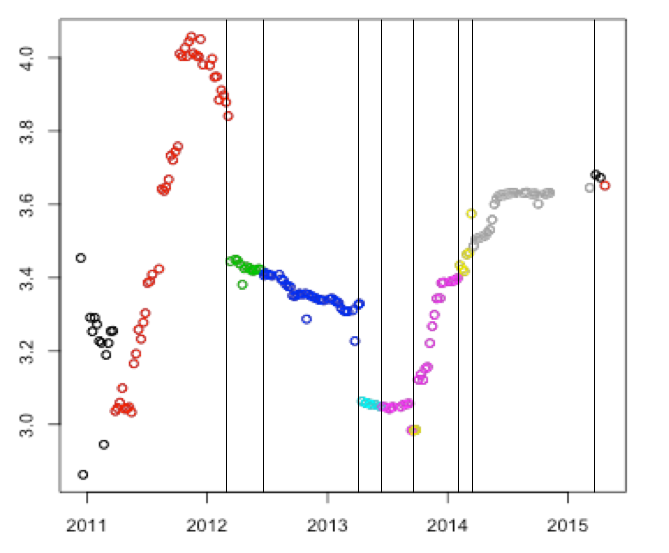
\includegraphics[width=\linewidth]{figs/model1.png}
\end{minipage}
\begin{minipage}{.45\linewidth}
\centering
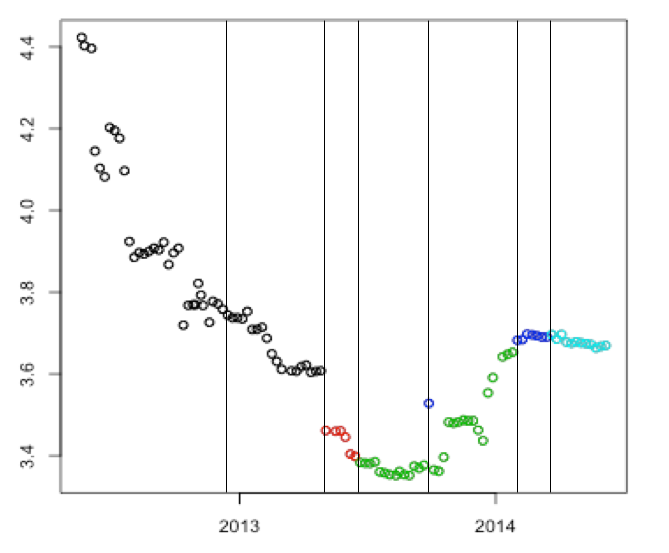
\includegraphics[width=\linewidth]{figs/model2.png}
\end{minipage}
\begin{minipage}{.45\linewidth}
\centering
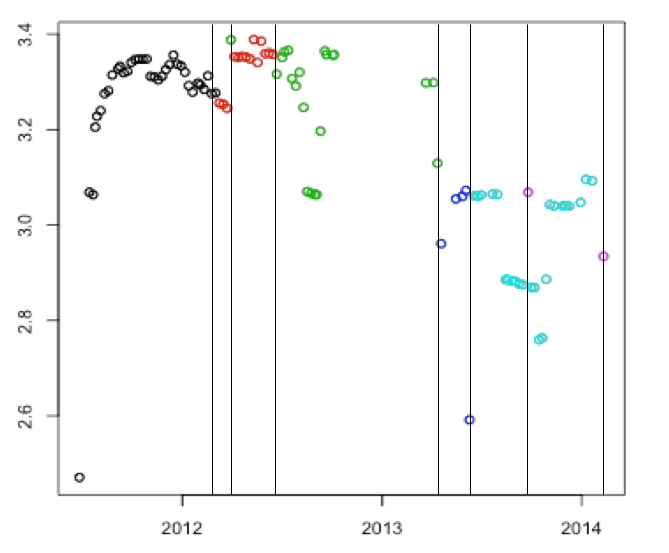
\includegraphics[width=\linewidth]{figs/model3.png}
\end{minipage}
\caption{Changes in model version with associated maintainability scores.}
\label{fig:model_inf}
\end{figure}

However, our most important findings did not involve the lifecycle stages of the systems. In figure \ref{fig:model_inf} we can see jumps in maintainability score which are not caused by large time differences between snapshots or lifecycle stage of the system but rather coincide with changes in SIG's maintainability model which are illustrated by vertical lines in the graphs. 

SIG uses the metrics in the snapshots to feed a proprietary model that processes and aggregates them to allow SIG to report on the system under review. To gain more insight into the specifics of the systems the model also generates new, composite metrics that are then added to the snapshot that is stored in the database. However, because SIG's model get periodically re-calibrated the version of the model used to generate a maintainability score and the composite metrics can differ between snapshots in ways that are not explainable by other factors such as time. This means that if we want to compare values of metrics between snapshots we have to ensure that all the snapshots were taken with the same model.

Table \ref{system} gives a short summary of the dataset. 
\begin{table}[htbp!]
\caption{Properties of Dataset}
\begin{tabular}{ l  p{4.8cm} }
  \hline			
  Property & Description \\ \hline
  Number of Systems & \textgreater1500 \\ 
  Number of Snapshots & $\sim$50000\\ 
  Median Snapshots Distance & 7 days\\ 
  Industries & Government, Insurance, Automotive, Commerce, Finance, Banking, Logistics, Telecom, Utility\\
  Attributes & Maintainability, Volume, Complexity, Total Lines of Code, New lines, Changed lines, Code Churn, Deleted lines, ...\\ \hline
\end{tabular}
\label{system}
\end{table}\\

Distribution analysis (see Figure \ref{fig:distrib}) showed that maintainability and unit complexity are nearly normally distributed with a mean of 3.32. and 3.36 respectively. Volume ratings are however left-skewed with a median of 4.8 and a the 10th percentile at 2.8. Lines of code and code churn are accordingly right-skewed. 

\begin{figure}[htb]
\centering
\begin{minipage}{.45\linewidth}
\centering
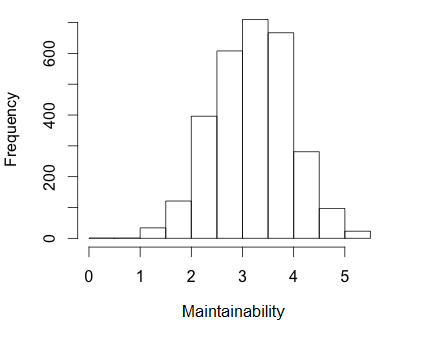
\includegraphics[width=\linewidth]{figs/Rplot__sval.png}
\end{minipage}
\caption{Histograms and Q-Q Plots of Maintainability and Volume distributions in the given data set.}
\label{fig:distrib}
\end{figure}

Correlation analysis showed that complexity and maintainability have a Person's correlation of 0.86, based which was decided to exclude unit complexity from further analysis because of information redundancy with maintainability. Volume and lines of code showed an expected high negative correlation of -0.97 Spearman's rho, but lines of code were kept in the dataset for eventual relative churn calculations. Furthermore, volume showed a 0.63 Spearman's rho correlation with maintainability and a -0.42 Spearman's rho correlation with code churn. We can conclude that we have to take interaction effects between volume, maintainability and churn for further analysis into account.

%%% Local Variables:
%%% mode: latex
%%% TeX-master: "IWSM-Mensura-2016"
%%% End:
